\documentclass[11pt]{article}

\usepackage{graphicx, epsfig}
\usepackage{amsmath, amssymb, latexsym}
\usepackage[english]{babel}
\usepackage{amssymb}   
%\usepackage{graphicx}
%\usepackage{float} 






% Make a larger page (shrink the margins)
%
\setlength{\textwidth}{6.7in}
\setlength{\textheight}{9.0in}
\setlength{\evensidemargin}{0.0in}
\setlength{\oddsidemargin}{0.0in}
\topmargin -0.5in
\footskip 0.5in



\title{Weekly Report for August 10th}
\author{Eric Davis}
\begin{document}
\maketitle
\medskip



\section{Comparing Filters}
\hspace{0.5cm}

This week I started looking for correlations between wavelength and the heights of Jupiter's Gaussian time profile above the background noise. I included them in this report for completeness as you have already seen them. The normalized counts for the various nights correspond very well together, and according to Craig they are as good a results as can be expected. The only outliers seem to appear in the Fort Smith November plot. The November 16th data for the 6250 and 6300 Angstrom wavelengths have an unusually high amplitude, but everything else is consistent. As well, there is the characteristic dip present in all plots at 4861 Angstroms, as expected.

\begin{figure}[h!]
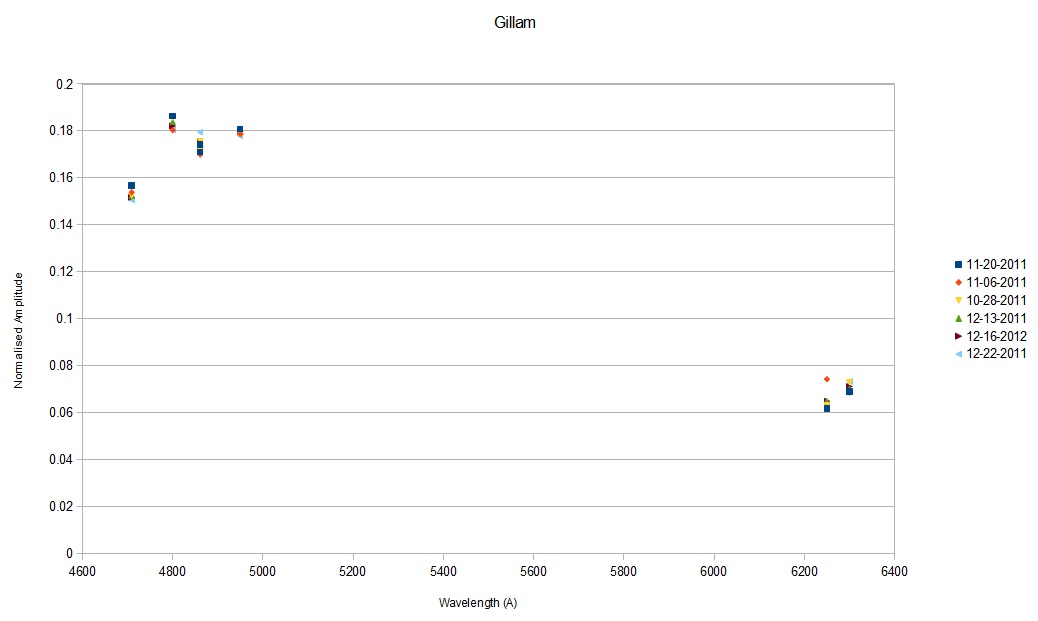
\includegraphics[scale=0.6]{norm_gillam.jpg}
\end{figure}

\begin{figure}[h!]
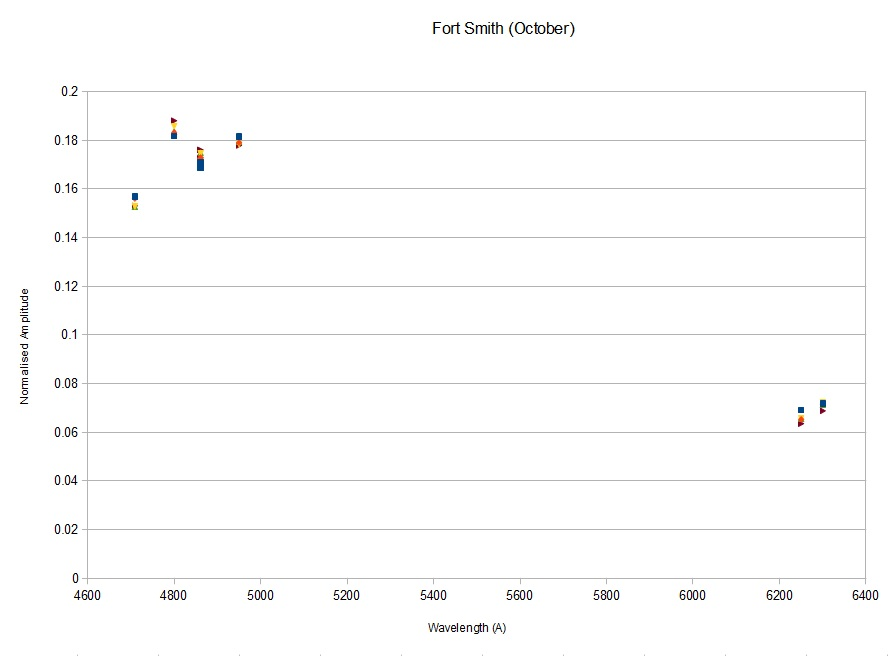
\includegraphics[scale=0.6]{norm_fortsmith_october.jpg}
\end{figure}

\begin{figure}
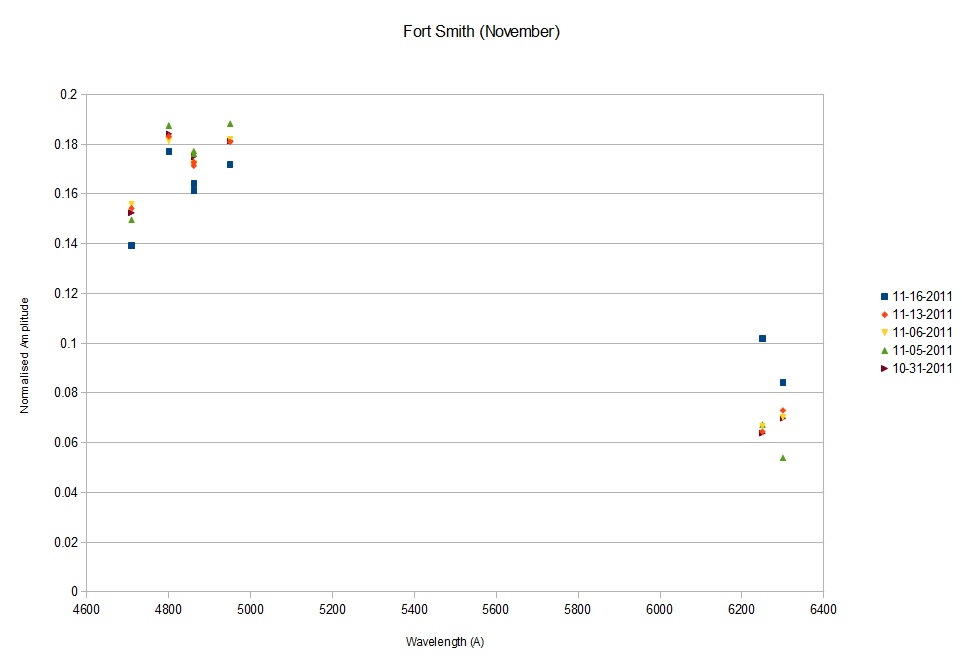
\includegraphics[scale=0.6]{norm_fortsmith_november.jpg}
\end{figure}

\begin{figure}
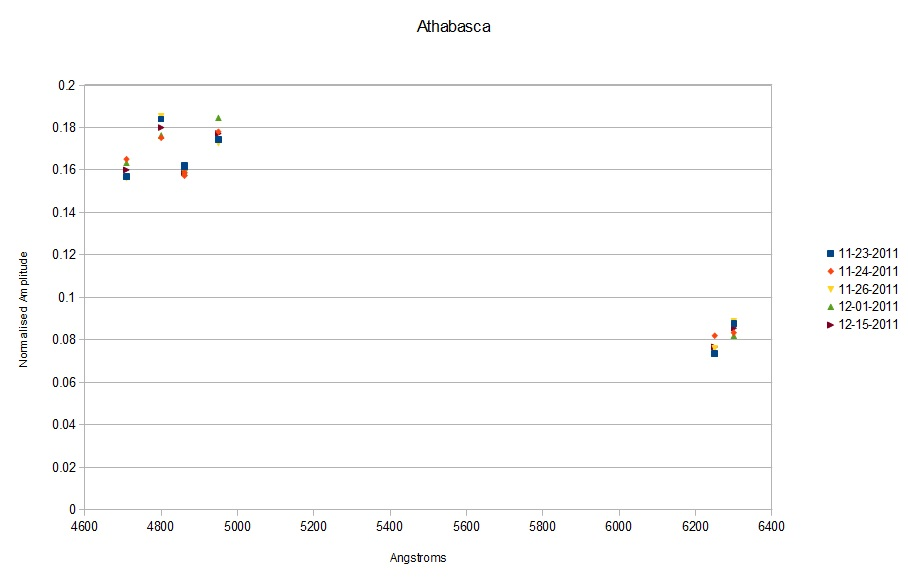
\includegraphics[scale=0.6]{norm_athabasca.jpg}
\end{figure}

\begin{figure}
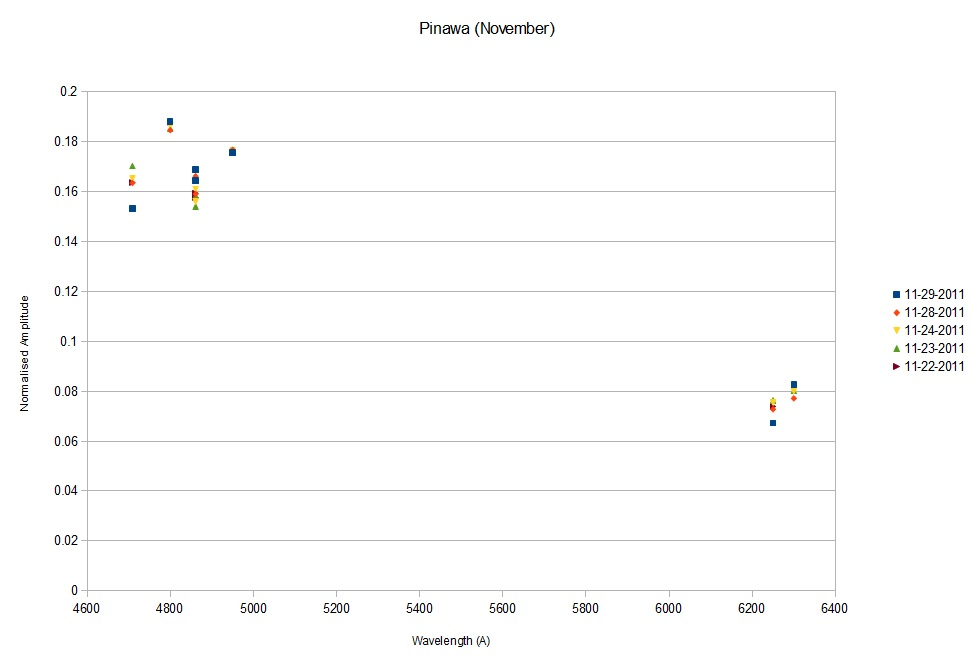
\includegraphics[scale=0.6]{norm_pinawa_november.jpg}
\end{figure}

\begin{figure}
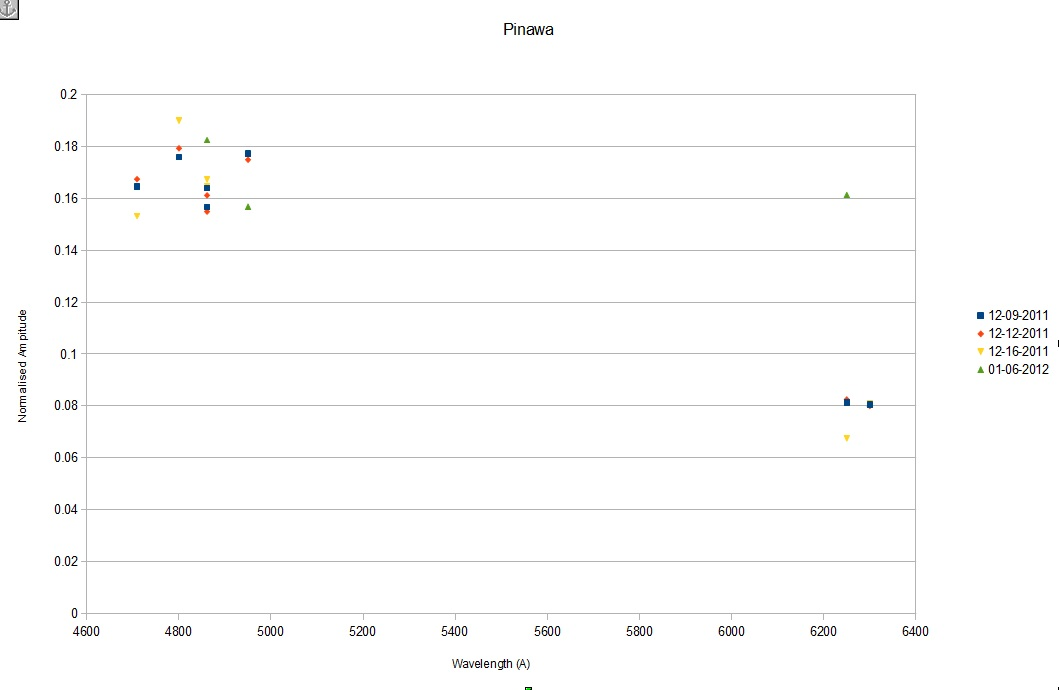
\includegraphics[scale=0.6]{norm_pinawa_december.jpg}
\end{figure}

\vspace{10mm}

\section{Space Profiles}
\hspace{0.5cm}

I started compiling a spread sheet for Fort Smith for the transit column and transit time. However, the process was a tad slow for obtaining accurate times. I have improved my code a bit to help with this and should go quite a bit smoother for the other sites. As of right now I am still in the process of compiling enough data to be able to map the direction of the cameras. 



\section{Future Considerations}
\hspace{0.5cm}

Next week I will look at the step table data you gave me and hopefully be able to transfer the transit columns into physical values. I plan to try and get it done for Fort Smith before moving on to collect the necessary data from the other sites. I want to have at least five points that at least five months apart for all four sites. I believe if it is good data it should be enough to get the job done.

\end{document}
\end{article}